\documentclass[10pt,twocolumn,a4paper]{article}
\usepackage[utf8]{inputenc}
\usepackage[T1]{fontenc}
\usepackage{amsmath,amssymb,amsfonts}
\usepackage{graphicx}
\usepackage{booktabs}
\usepackage{hyperref}
\usepackage{caption}
\usepackage{cite}
\usepackage[margin=0.75in]{geometry}
\usepackage{algorithm}
\usepackage{algorithmic}
\usepackage{subcaption}
\usepackage{xcolor}
\usepackage{enumitem}

%==============================================================================
\title{\bf Why Neural Heuristics Fail in IDA* Search:\\ A Case Study on Rubik's Cube with Practical Solutions}
%==============================================================================
\author{Anonymous Author(s)\\ \textit{Department / Institution}\\ \texttt{author@example.com}}
\date{}

\begin{document}
\maketitle

%==============================================================================
\begin{abstract}
The Rubik's Cube has approximately $4.3 \times 10^{19}$ reachable states, making exhaustive optimal search impractical. We present a \emph{practical} solver based on Kociemba's Two-Phase Algorithm with three categories of improvement: (i)~\textbf{multi-solution Phase~1 search}, which explores multiple Phase~1 endpoints and retains the shortest combined solution; (ii)~\textbf{time-bounded anytime mode}, which returns the best solution found within a fixed time budget; and (iii)~\textbf{neural heuristic integration strategies} that address a fundamental problem: na\"ive neural lower bounds cause IDA* to search exponentially more nodes due to the ``admissible bound paradox.'' We show that the correct integration is through \emph{move ordering}, not bound tightening, and propose three strategies (always, probabilistic, depth-adaptive). On 200 random cubes (seed 42), multi-solution search with $K=5$ reduces mean move count from 20.77 to 20.30 ($p < 0.001$, Cohen's $d = 0.75$) and increases the fraction of $\leq$20-move solutions from 28\% to 60.5\%. However, we report a significant \emph{negative result}: all three neural ordering strategies produce no measurable improvement over the non-neural baseline. We verify this with two training paradigms (inverse-move labels: $\sim$5.6\% accuracy; solver-feedback labels: 3.9\%, \emph{below} random), concluding that the bottleneck is the state representation itself (one-hot facelets), not training signal quality or integration architecture. We instrument the solver with node expansion counters and provide paired statistical tests for rigorous comparison. The benchmark infrastructure, trained neural models, and reproducible result JSON files are provided.
\end{abstract}

\noindent\textbf{Index Terms---}Rubik's Cube, two-phase algorithm, Kociemba, IDA*, pruning tables, neural heuristics, move ordering, anytime solver, multi-solution search.
\vspace{0.5em}

%==============================================================================
\section{Introduction}
\label{sec:intro}
%==============================================================================

\subsection{Background}
The Rubik's Cube, invented by Ern\H{o} Rubik in 1974, has become a standard testbed for combinatorics, group theory, and heuristic search. Its configuration space forms a group under face turns; the six faces (Up, Down, Left, Right, Front, Back) generate the group via quarter and half turns. A single standard $3{\times}3{\times}3$ cube has 26 visible sub-cubes (cubies): 8 corners, 12 edges, and 6 face centers. Each corner has 3 visible faces (stickers) and each edge has 2, giving 54 total stickers---the natural input to any computational representation.

The mathematical structure of the cube is remarkably rich. The group of reachable configurations has order
\begin{equation}
|G| = \frac{8! \cdot 3^8 \cdot 12! \cdot 2^{12}}{12} \approx 4.33 \times 10^{19},
\end{equation}
where the factors account for corner permutations ($8!$), corner orientations ($3^8$), edge permutations ($12!$), and edge orientations ($2^{12}$), with a factor-of-12 constraint from parity and orientation sum rules. This enormous state space makes exhaustive enumeration or brute-force search completely impractical.

\subsection{Problem Statement: God's Number}
``God's Number'' is the minimum number of moves required to solve any solvable cube from worst-case positions. In the \emph{half-turn metric} (HTM), where both quarter turns ($U$, $U'$) and half turns ($U2$) each count as one move, God's Number is \textbf{20}. Rokicki et al.\ proved this in 2010 by combining group-theoretic coset decomposition with massive distributed computation (35 CPU-years on Google infrastructure). In the \emph{quarter-turn metric} (QTM), where each $90^\circ$ turn counts separately, God's Number is \textbf{26}.

The practical implication is clear: \emph{every} scrambled cube can be solved in at most 20 half-turn moves. However, finding these optimal solutions requires exhaustive search through the vast state space, which is infeasible in real time. This motivates the use of near-optimal algorithms that sacrifice guaranteed optimality for vastly improved speed.

\subsection{Motivation and Contributions}
Kociemba's Two-Phase Algorithm offers a practical compromise: it does not guarantee 20 moves for every instance but typically produces 19--22 move solutions in a fraction of a second. It improves on Thistlethwaite's four-phase method by using two phases and efficient coordinate-based search with pruning tables. This work implements the algorithm and adds three categories of extension:

\begin{enumerate}[leftmargin=*]
  \item \textbf{Multi-solution Phase~1 search} ($K > 1$ endpoints), which explores multiple Phase~1 exit points and retains the shortest combined solution.
  \item \textbf{Time-bounded anytime mode}, which caps solve latency for interactive applications while returning the best solution found within the budget.
  \item \textbf{Neural heuristic integration strategies} that address a fundamental problem we identify (the ``admissible bound paradox'') and propose three architecturally sound alternatives.
\end{enumerate}

The contribution is aimed at application and systems-oriented venues. We provide:
\begin{itemize}[leftmargin=*]
  \item Recommended settings with statistical validation ($K{=}5$, 0.5\,s budget).
  \item Quantitative trade-offs (move count vs.\ time, solution quality vs.\ budget).
  \item A principled analysis of why na\"ive neural bounds fail in IDA*.
  \item A documented negative result on neural move ordering with shallow MLPs.
  \item Full open reproducibility (seed, scripts, JSON outputs).
\end{itemize}

\subsection{Paper Organization}
Section~\ref{sec:related} reviews related work on optimal solvers, learning-based approaches, and neural heuristics in planning. Section~\ref{sec:math} presents the mathematical foundation of the Two-Phase Algorithm. Section~\ref{sec:method} details our methodology including multi-solution search, anytime mode, and neural integration strategies. Section~\ref{sec:setup} describes the experimental setup. Sections~\ref{sec:results} and~\ref{sec:discussion} present and discuss experimental results. Section~\ref{sec:conclusion} concludes with contributions and Section~\ref{sec:future} outlines future directions.

%==============================================================================
\section{Related Work}
\label{sec:related}
%==============================================================================

\textbf{Optimal solvers and God's Number.}
Korf~\cite{korf1997} achieved the first optimal solver for Rubik's Cube using IDA* with pattern databases, proving specific instances require 18 moves. His approach used additive pattern databases to construct admissible heuristics, establishing the template for optimal combinatorial puzzle solving. Rokicki et al.~\cite{godnumber} proved God's Number is 20 in the half-turn metric by combining group-theoretic coset decomposition with massive computation (35 CPU-years on Google infrastructure). Their work partitioned the $4.3 \times 10^{19}$ states into $\sim$2.2 billion cosets and showed that each coset can be solved in $\leq$20 moves, establishing the theoretical ceiling that practical solvers aim toward.

\textbf{Thistlethwaite and Kociemba.}
Thistlethwaite's algorithm~\cite{thistlethwaite1981} reduces the cube to the identity through four nested subgroups, each restricting the allowed moves. The chain $G_0 \supset G_1 \supset G_2 \supset G_3 \supset \{e\}$ progressively constrains the cube until only the identity remains. Kociemba~\cite{kociemba} simplified this to two phases---first reducing the cube to a subgroup $G_1$ (fixing edge orientation, corner orientation, and equatorial slice) and then solving within $G_1$---yielding near-optimal solutions in milliseconds via precomputed pruning tables. The key insight is that the two-phase decomposition reduces a 20-move search in a branching-factor-18 space to two shorter searches in smaller spaces, making real-time solving practical. Our work builds on Kociemba's algorithm and extends it with multi-solution Phase~1 search ($K$ endpoints) and time-bounded anytime mode.

\textbf{Deep learning for combinatorial puzzles.}
Agostinelli et al.~\cite{deepcubea} introduced DeepCubeA, which uses deep approximate value iteration and weighted A* to solve Rubik's Cube optimally in 60\% of cases, with median solution length of 21. Their network (a ResNet with $\sim$500K parameters) trains on randomly scrambled cubes at increasing depths and learns a value function $v(s) \approx h^*(s)$ that guides A* search. The key advantage over classical pattern databases is that the neural value function can generalize across the state space without explicit enumeration. However, DeepCubeA requires $\sim$2 days of GPU training and $\sim$10 seconds per solve---orders of magnitude slower than Kociemba's algorithm. McAleer et al.~\cite{mcaleer2018} explored policy gradient methods (approximate policy iteration) for the cube but found them less effective than value-based approaches, achieving comparable optimality rates but with higher variance. Brunetto and Trunda~\cite{brunetto2017} applied CNNs to estimate the distance-to-goal for the 15-puzzle and Rubik's Cube, reporting that cube-specific architectures are needed for good generalization---a finding consistent with our negative result on shallow MLPs with generic facelet encodings.

\textbf{Neural heuristics in classical planning.}
Beyond puzzles, learned heuristics have been applied to classical planning domains. Shen et al.~\cite{shen2020} trained neural networks to approximate the $h^*$ heuristic for IDA*, finding that even small approximation errors can cause exponential node expansion increases---a phenomenon they call the ``heuristic noise'' problem. Their analysis shows that an $\epsilon$-error in the heuristic can increase the effective solution depth by $O(\epsilon \cdot d)$ iterations in IDA*, each of which expands exponentially more nodes. Ferber et al.~\cite{ferber2022} studied neural network heuristics in STRIPS planning and showed that informative features and sufficient training data are critical; architectures with domain-specific inductive biases (e.g., graph convolutions over the problem structure) outperform generic MLPs. Our work provides a concrete case study of this failure mode: we demonstrate that shallow MLPs on one-hot facelet encodings produce near-uniform predictions, rendering neural move ordering ineffective regardless of integration strategy.

\textbf{Layer-by-Layer (LBL) methods.}
Human-oriented methods solve the cube in stages (cross, first layer, second layer, OLL, PLL). Move count is high (often 80--120 moves), but the method is easy to learn and execute by hand. Speed-cubing methods like CFOP~\cite{fridrich} reduce move counts to 50--60 on average through memorized algorithm sets, achieving sub-10-second solves for expert humans. The gap between CFOP's $\sim$55 moves and Kociemba's $\sim$20 moves illustrates the power of algorithmic search over memorized procedures.

\textbf{Positioning.}
Our work differs from DeepCubeA and similar end-to-end learned solvers in that we study neural heuristics as \emph{add-ons} to an established classical algorithm (Kociemba two-phase). This is a practically relevant scenario---augmenting a reliable, fast solver with learned guidance---and our negative results highlight the difficulty of this integration even when the architecture is carefully designed to preserve admissibility. While DeepCubeA demonstrates that deep networks \emph{can} learn cube heuristics with sufficient capacity and training, our results show that shallow networks with impoverished representations \emph{cannot}, even when integrated via principled strategies that avoid the admissible bound paradox.

%==============================================================================
\section{Mathematical Foundation}
\label{sec:math}
%==============================================================================

The set of reachable states of the Rubik's Cube forms a group $G$ under the operation of applying one move after another. The full group is generated by the six face turns:
\begin{equation}
G_0 = \langle U, D, L, R, F, B \rangle.
\end{equation}
Each generator admits three non-trivial moves: a clockwise quarter turn ($X$), a half turn ($X^2$), and a counter-clockwise quarter turn ($X' = X^3$). This gives $6 \times 3 = 18$ possible moves at each state, establishing the branching factor for search.

\subsection{Coordinate System}
\label{sec:coordinates}
Rather than storing full permutation arrays, the solver encodes each cube state using compact \emph{coordinates} that capture the relevant symmetry properties:

\begin{itemize}[leftmargin=*]
  \item \textbf{Twist} ($0 \leq \text{twist} < 2187 = 3^7$): Encodes the orientation of 8 corners (the 8th is determined by the others).
  \item \textbf{Flip} ($0 \leq \text{flip} < 2048 = 2^{11}$): Encodes the orientation of 12 edges (the 12th is determined).
  \item \textbf{Slice} ($0 \leq \text{slice} < 495 = \binom{12}{4}$): Encodes which 4 of 12 edge positions are occupied by middle-slice edges.
  \item \textbf{URFtoDLF} ($0 \leq c < 20160 = 8!/2$): Corner permutation coordinate for Phase~2.
  \item \textbf{URtoDF} ($0 \leq c < 665280 = 12!/(12{-}6)!$): Six-edge permutation coordinate for Phase~2.
\end{itemize}

Moves are applied by table lookup: for each coordinate $c$ and move $m$, a precomputed table stores the resulting coordinate $c' = \text{moveTable}[c][m]$. This reduces each move application to $O(1)$ table lookups.

\subsection{Phase~1: Target Subgroup $G_1$}
Phase~1 searches for a path from the initial state (in $G_0$) to a state in the subgroup
\begin{equation}
G_1 = \langle U, D, L^2, R^2, F^2, B^2 \rangle.
\end{equation}
A state belongs to $G_1$ if and only if: (i)~all 12 edges have correct orientation (flip $= 0$), (ii)~all 8 corners have correct orientation (twist $= 0$), and (iii)~the four middle-slice edges occupy middle-slice positions (slice $= 0$). The combined Phase~1 coordinate space has size $2187 \times 2048 \times 495 \approx 2.2 \times 10^9$.

\subsection{Pruning Tables}
\label{sec:pruning}
Pruning tables store the minimum number of moves to reach $G_1$ (or the identity, in Phase~2) from each coordinate value. They are computed by backward BFS from the target:

\begin{itemize}[leftmargin=*]
  \item \textbf{Slice--Twist pruning} ($495 \times 2187$): Lower bound from slice and twist coordinates.
  \item \textbf{Slice--Flip pruning} ($495 \times 2048$): Lower bound from slice and flip coordinates.
  \item \textbf{Phase~2 pruning}: Uses URFtoDLF, URtoDF, and the restricted slice coordinate.
\end{itemize}

The admissible heuristic at any node is $h = \max(h_{\text{slice-twist}}, h_{\text{slice-flip}})$ for Phase~1. This maximum of two projections provides a tighter lower bound than either alone while remaining admissible (since both are lower bounds on the true distance).

\subsection{Phase~2}
From any state in $G_1$, only the 10 moves from the generating set of $G_1$ are used: $\{U, U', U^2, D, D', D^2, L^2, R^2, F^2, B^2\}$. Phase~2 finds a path to the identity (solved cube). The restricted move set keeps the effective branching factor at $\sim$10 (vs.\ 18 in Phase~1) and allows strong pruning via precomputed tables, making Phase~2 searches typically much cheaper than Phase~1.

\subsection{IDA* Search}
\label{sec:ida-star}
Both phases use Iterative Deepening A* (IDA*). IDA* performs a series of depth-limited depth-first searches with increasing cost thresholds. At each node with depth $g$ and heuristic estimate $h$, the node is pruned if $f = g + h > d_{\text{limit}}$. The threshold $d_{\text{limit}}$ starts at $h(\text{root})$ and increases to the minimum $f$-value that exceeded the previous limit. This provides the optimality guarantees of A* with $O(d)$ memory (where $d$ is the solution depth), at the cost of re-expanding some nodes across iterations.

The critical property for our analysis: the number of nodes expanded by IDA* grows \emph{exponentially} with $d_{\text{limit}}$. If the branching factor is $b$, iteration $d$ expands $O(b^d)$ nodes. This means that increasing the effective depth threshold by even one move multiplies the work by $\sim b$.

%==============================================================================
\section{Methodology and Implementation}
\label{sec:method}
%==============================================================================

\begin{figure}[t]
  \centering
  \begin{subfigure}{0.31\columnwidth}
    \centering
    \includegraphics[width=\linewidth]{figures/ui_input_1.png}
  \end{subfigure}\hfill
  \begin{subfigure}{0.31\columnwidth}
    \centering
    \includegraphics[width=\linewidth]{figures/ui_input_2.png}
  \end{subfigure}\hfill
  \begin{subfigure}{0.31\columnwidth}
    \centering
    \includegraphics[width=\linewidth]{figures/ui_input_3.png}
  \end{subfigure}

  \vspace{0.35em}

  \begin{subfigure}{0.31\columnwidth}
    \centering
    \includegraphics[width=\linewidth]{figures/ui_input_4.png}
  \end{subfigure}\hfill
  \begin{subfigure}{0.31\columnwidth}
    \centering
    \includegraphics[width=\linewidth]{figures/ui_input_5.png}
  \end{subfigure}
  \caption{User interaction snapshots during face selection and guided sticker entry.}
  \label{fig:ui_input_sequence}
\end{figure}

\subsection{System Architecture}
The solver uses two representations:
\begin{itemize}[leftmargin=*]
  \item \textbf{Facelet level:} A string of 54 characters (U1--U9, R1--R9, F1--F9, D1--D9, L1--L9, B1--B9) representing the color of each sticker. This representation is used for I/O, user interfaces, and as input to the neural heuristic.
  \item \textbf{Cubie/coordinate level:} Corner and edge permutation/orientation and slice coordinates (Section~\ref{sec:coordinates}). Moves are applied as permutations via table lookup; pruning tables are indexed by these coordinates.
\end{itemize}

The translation from facelet string to cubie representation is performed once at the start of each solve. The reverse translation is not needed during search---only the coordinate representation is used for move application and pruning.

\subsection{Proposed Improvements}
\label{sec:improvements}

We implement and evaluate three categories of extensions to the baseline Two-Phase solver.

\subsubsection{Multi-Solution Phase~1 Search}
\label{sec:multi-phase1}

\textbf{Rationale.} The baseline Kociemba solver returns the \emph{first} Phase~1 solution found, then runs Phase~2 once. The length of the final solution depends on the particular Phase~1 path chosen; many cubes admit several distinct Phase~1 endpoints, and the corresponding Phase~2 solutions can differ significantly in length. By exploring multiple Phase~1 solutions and running Phase~2 for each, we can keep the shortest combined solution.

\textbf{Algorithm.} We introduce a parameter \texttt{max\_phase1\_solutions} $K \geq 1$. The Phase~1 IDA* search is unchanged except that whenever a state in $G_1$ is reached:
\begin{enumerate}
  \item Phase~2 is run from that state to obtain a full solution and its move count $L$.
  \item If $L$ is shorter than the best so far, the solution and $L$ are stored.
  \item If fewer than $K$ Phase~1 solutions have been processed, the search continues to find more Phase~1 endpoints; otherwise it terminates and returns the best solution.
\end{enumerate}
Thus for $K=1$ the behavior is identical to the baseline (first solution only). For $K>1$, the solver invests more time in Phase~1 to discover alternative paths into $G_1$, trading compute time for shorter solutions. No change to Phase~2 or to the pruning tables is required.

The pseudocode for multi-solution Phase~1 IDA* is given in Algorithm~\ref{alg:multi-phase1}.

\begin{algorithm}[t]
\caption{Multi-Solution Phase~1 IDA*}
\label{alg:multi-phase1}
\begin{algorithmic}[1]
\REQUIRE Cube state $s_0$, max solutions $K$, time budget $T$
\ENSURE Best solution found
\STATE $d_{\text{limit}} \gets h_1(s_0)$
\STATE $\text{best} \gets \text{None}$; $\text{best\_len} \gets \infty$; $\text{count} \gets 0$
\WHILE{$\text{count} < K$ \AND elapsed $< T$}
  \STATE $t \gets$ \textsc{DFS-Phase1}($s_0$, $0$, $d_{\text{limit}}$)
  \IF{$t = \text{FOUND}$}
    \STATE \textbf{continue} \COMMENT{Phase~1 found endpoint; DFS-Phase1 updates best}
  \ENDIF
  \IF{$t = \infty$}
    \STATE \textbf{break} \COMMENT{No more solutions exist}
  \ENDIF
  \STATE $d_{\text{limit}} \gets t$ \COMMENT{Increase threshold}
\ENDWHILE
\RETURN best
\end{algorithmic}
\end{algorithm}

\begin{algorithm}[t]
\caption{\textsc{DFS-Phase1}($s$, $g$, $d_{\text{limit}}$)}
\label{alg:dfs-phase1}
\begin{algorithmic}[1]
\STATE $h \gets \max(h_{\text{slice-twist}}(s),\; h_{\text{slice-flip}}(s))$
\STATE $f \gets g + h$
\IF{$f > d_{\text{limit}}$}
  \RETURN $f$ \COMMENT{Pruned---return next threshold}
\ENDIF
\IF{$h = 0$} \COMMENT{$s \in G_1$}
  \STATE $L \gets$ Phase2Solve($s$) + $g$
  \IF{$L < \text{best\_len}$}
    \STATE $\text{best} \gets$ solution; $\text{best\_len} \gets L$
  \ENDIF
  \STATE $\text{count} \gets \text{count} + 1$
  \RETURN FOUND
\ENDIF
\STATE $\text{min\_t} \gets \infty$
\STATE moves $\gets$ \textsc{OrderMoves}($s$, $g$) \COMMENT{Neural or default}
\FOR{each move $m$ in moves}
  \STATE $s' \gets$ applyMove($s$, $m$)
  \STATE $t \gets$ \textsc{DFS-Phase1}($s'$, $g{+}1$, $d_{\text{limit}}$)
  \STATE $\text{min\_t} \gets \min(\text{min\_t}, t)$
\ENDFOR
\RETURN $\text{min\_t}$
\end{algorithmic}
\end{algorithm}

\textbf{Implementation detail.} The existing Python solver already supports $K>1$: it maintains \texttt{best\_solution} and \texttt{best\_length} and, in the Phase~1 loop, compares each new full solution length against \texttt{best\_length} before updating. The application layer previously called the solver with default $K=1$; we expose $K$ in the API and set $K=5$ (and optionally a time budget) for the 3D interface.

\subsubsection{Time-Bounded Anytime Mode}
\label{sec:anytime}

\textbf{Rationale.} In interactive applications (e.g., a 3D cube interface), unbounded solve time is unacceptable. Multi-solution search can increase solve time significantly; we need a way to cap latency while still returning a valid, preferably short, solution.

\textbf{Design.} We add an optional parameter \texttt{time\_budget\_sec} $T \geq 0$ (e.g., $T = 0.5$ seconds). Before each iteration of the Phase~1 search loop, we check whether elapsed time since the start of the solve exceeds $T$. If it does:
\begin{itemize}
  \item If at least one full solution has been found, the solver returns that best solution immediately (anytime behavior).
  \item If no solution has been found yet, the solver raises a timeout exception so the caller can handle it (e.g., retry with a longer budget or fall back to a faster setting).
\end{itemize}
No threading is required: the search is single-threaded, and the time check is performed at the existing loop re-entry point where \texttt{time.time()} is already used for timeout handling.

\textbf{Analysis.} The anytime property is monotone: the best solution length is non-increasing over time. Early in the search, the solver finds a solution quickly (often within 100\,ms) and then progressively discovers shorter alternatives. The time budget thus provides a tunable quality-latency knob: short budgets (0.1\,s) return the first solution found, while longer budgets (1.0\,s) allow exploration of multiple Phase~1 endpoints.

\textbf{Integration with multi-solution search.} When \texttt{time\_budget\_sec} is set, \texttt{max\_phase1\_solutions} can be set to a relatively high value (e.g., 20) so that the solver keeps exploring Phase~1 solutions until the budget is exhausted, then returns the best solution found. This yields a predictable maximum latency (e.g., 500\,ms) while still improving over the first-solution-only result when time permits.

\subsubsection{Neural Heuristic Integration Strategies}
\label{sec:neural-strategies}

\textbf{Problem: Why Na\"ive Neural Heuristics Fail in IDA*.}
A natural idea is to train a neural network to predict moves or lower bounds and use it to speed up search. However, na\"ive integration fails for a subtle reason specific to IDA*. In IDA*, the depth threshold $d$ increases by~1 each iteration, and the number of nodes expanded grows \emph{exponentially} with $d$. If a neural value predictor produces a bound $h_{\mathrm{nn}}$ that is sometimes stronger than the pruning table bound $h_{\mathrm{pt}}$, the effective heuristic
\begin{equation}
h_{\text{eff}}(s) = \max\bigl(h_{\mathrm{pt}}(s),\; h_{\mathrm{nn}}(s)\bigr)
\label{eq:max-heuristic}
\end{equation}
can increase the depth at which the optimal solution is first found, causing IDA* to search exponentially more nodes. Concretely, if $h_{\mathrm{nn}}$ overestimates the true distance for even a small fraction of states along the optimal solution path, the IDA* threshold must be raised, adding entire iterations of exponential cost. We observed up to 133$\times$ slowdown when using the neural bound under the MAX combining rule of Eq.~\eqref{eq:max-heuristic}.

\textbf{Key insight.} The correct way to integrate learned information into IDA* is to use neural predictions for \emph{move ordering} within a fixed depth threshold, not to tighten the admissible lower bound. This preserves the depth threshold sequence (and thus the total number of iterations) but reduces the \emph{effective} branching factor by exploring more promising moves first within each iteration.

\textbf{Three strategies.} We implement and evaluate three neural integration strategies, all of which use the neural move predictor for \emph{ordering} only and leave the pruning-table bound unchanged:

\begin{enumerate}[leftmargin=*]
  \item[\textbf{(A)}] \textbf{Move Ordering (always):} At every node, query the neural move predictor $\pi_\theta(s)$ for a probability distribution over the 18 moves and sort them in descending order of predicted probability. This biases the search toward moves the network considers most promising. The computational overhead is one forward pass per node.
  \item[\textbf{(B)}] \textbf{Probabilistic Sampling:} At each node, use the neural ordering with probability $p$ and the default fixed ordering with probability $1-p$. This adds diversity: when the neural model is inaccurate, we still explore the original order frequently enough to avoid pathological cases. The parameter $p$ controls the influence: $p=0$ recovers baseline, $p=1$ recovers Strategy~A.
  \item[\textbf{(C)}] \textbf{Adaptive Depth Cutoff:} Use neural ordering only at depths $\leq D_{\mathrm{cut}}$ (e.g., $D_{\mathrm{cut}} = 5$) and revert to the default ordering for deeper nodes. Rationale: at shallow depths, the cube is far from solved and move ordering can steer the search effectively; at deep depths (near the goal), the pruning tables are already highly informative and the network adds overhead without benefit.
\end{enumerate}

All three strategies preserve admissibility and completeness of IDA*---only the node expansion order changes, not the depth threshold or the pruning bound. This is formalized in Proposition~\ref{prop:completeness}.

\begin{proposition}[Completeness Preservation]
\label{prop:completeness}
Let $\sigma$ be any permutation of the 18 moves applied at each node in the IDA* DFS. The search with ordering $\sigma$ visits the same set of nodes within each depth-limited iteration as the default ordering and hence finds all solutions that the default search finds.
\end{proposition}

\begin{proof}
Within each iteration (fixed $d_{\text{limit}}$), IDA* performs a complete depth-first traversal of all nodes with $f \leq d_{\text{limit}}$. Reordering children of a node changes only the \emph{order} of traversal, not the \emph{set} of nodes visited. Since the IDA* framework explores all children at each non-pruned node and the pruning criterion ($f > d_{\text{limit}}$) is independent of traversal order, the same nodes are expanded regardless of ordering. Thus optimality and completeness are preserved. \qed
\end{proof}

\subsection{Neural Network Architecture}
\label{sec:neural-arch}

We train two neural network models:

\textbf{Move Predictor} ($\pi_\theta$): A multi-layer perceptron (MLP) that takes the 54-dimensional one-hot facelet encoding as input and predicts a probability distribution over 18 moves. Architecture: $54 \times 6 = 324 \to 256 \to 128 \to 64 \to 18$ (with ReLU activations and softmax output). The one-hot encoding maps each of the 54 stickers to a 6-dimensional indicator vector (one per color), giving a $324$-dimensional input.

\textbf{Value Predictor} ($v_\phi$): An MLP that estimates the number of moves to solve: $324 \to 512 \to 256 \to 128 \to 1$ (with ReLU activations). This model is used only for analysis of the admissible bound paradox; it is \emph{not} used in any of the three strategies (A, B, C) which use only the move predictor.

\textbf{Training data.} We generate training cubes by applying $k$ random moves to the solved state ($k \sim \text{Uniform}[1, 25]$). The \emph{inverse-move} label for each state is the reverse of the last scramble move---a simple proxy for the ``best'' move. We also experiment with \emph{solver-feedback} labels, where the label is the first move of the Kociemba solver's actual solution (a stronger training signal but substantially more expensive to generate, since each training example requires a full solve).

\textbf{Training details.} 50,000 training cubes, batch size 64, Adam optimizer ($\text{lr} = 10^{-3}$), 30 epochs. Training time: $\sim$5 minutes on a laptop CPU for inverse-move labels, $\sim$2 hours for solver-feedback labels (dominated by solve time per sample).

\subsection{Instrumentation}
\label{sec:instrumentation}

To quantify the effect of these strategies, we instrument the search with per-solve counters:
\begin{itemize}[leftmargin=*]
  \item \textbf{Total nodes expanded}: Number of recursive DFS calls across all IDA* iterations.
  \item \textbf{Phase~1 nodes}: Subset of total nodes expanded during Phase~1 search.
  \item \textbf{Phase~2 nodes}: Subset during Phase~2 search.
  \item \textbf{Max depth reached}: Highest depth explored in any iteration.
  \item \textbf{Phase~1 endpoints found}: Number of distinct $G_1$ states reached.
  \item \textbf{Full solutions found}: Number of complete solutions (Phase~1 + Phase~2).
\end{itemize}

These counters are reset before each solve and returned alongside the solution string and solve time. This instrumentation enables paired statistical tests (same scramble, different strategy) rather than unpaired comparisons, substantially increasing statistical power.

\subsection{Statistical Methodology}
\label{sec:stats}

All strategy comparisons use the same set of scrambles (same random seed), enabling paired tests:
\begin{itemize}[leftmargin=*]
  \item \textbf{Paired $t$-test}: Tests whether the mean difference in move count (or node count) between two strategies is significantly different from zero. We report the $t$-statistic and $p$-value.
  \item \textbf{Cohen's $d$}: Effect size measure, computed as $d = \bar{\Delta} / s_\Delta$ where $\bar{\Delta}$ is the mean paired difference and $s_\Delta$ is its standard deviation. Conventionally, $d = 0.2$ is small, $d = 0.5$ medium, $d = 0.8$ large.
  \item \textbf{Bootstrap CI}: 95\% confidence intervals on the mean difference, computed via 10,000 bootstrap resamples of the paired differences.
\end{itemize}

\subsection{Technology Stack}
Python is used for the main solver and application; an optional C backend implements the same algorithm for lower latency. Libraries include a Python port of the Kociemba two-phase solver~\cite{muodov}, OpenCV for camera input, NumPy for numerical operations, PyTorch for neural network training and inference, and Matplotlib for 3D visualization, figure generation, and step-by-step playback. Cube input is via a 3D or 2D manual interface or camera-based face scanning; physical orientation is mapped to standard facelet order so solutions can be presented in user-oriented language (e.g., ``Turn the top face 90 degrees clockwise'').

%==============================================================================
\section{Experimental Setup}
\label{sec:setup}
%==============================================================================

\subsection{Hardware and Software}
All experiments were run on a consumer laptop (Apple M-series, 16\,GB RAM). The solver uses the pure Python backend for reproducibility; the C backend is available for deployment but not used in experiments. Python 3.11, NumPy 1.26, PyTorch 2.1, Matplotlib 3.8.

\subsection{Scramble Generation}
Random scrambles are generated by applying 25 random moves to the solved cube, using Python's \texttt{random.Random} with explicit seeds for reproducibility. We use seed 42 as the primary seed and seeds 123, 456, 789 for multi-seed validation. Each experiment uses 200 scrambles unless otherwise noted.

For hard-case analysis, we generate 50 scrambles: the superflip (a known maximally-hard configuration in certain metrics) plus 49 cubes obtained by applying 20 random moves to the solved state (seed 42). These 20-move-deep scrambles are expected to have optimal solutions near 20 moves, stressing the solver more than typical random scrambles (which average $\sim$20.77 moves in our baseline).

\subsection{Solver Configuration}
\begin{itemize}[leftmargin=*]
  \item \textbf{Timeout}: 5\,s per solve (no time budget) unless in anytime mode.
  \item \textbf{Pruning tables}: Precomputed and cached on first run ($\sim$30\,s to generate, $\sim$20\,MB on disk).
  \item \textbf{Neural model}: Loaded once at benchmark start; inference via PyTorch CPU forward pass.
\end{itemize}

\subsection{Benchmark Modes}
We evaluate the following experimental conditions:

\begin{enumerate}[leftmargin=*]
  \item \textbf{Baseline comparison} ($K{=}1$ vs.\ $K \in \{3, 5, 10\}$): 200 scrambles, seed 42.
  \item \textbf{Neural strategy comparison} (none, A, B, C with $K{=}5$): 200 scrambles, seed 42.
  \item \textbf{Probabilistic sweep} ($p \in \{0.1, 0.3, 0.5, 0.7, 0.9\}$ for Strategy~B): 200 scrambles, seed 42.
  \item \textbf{Anytime sweep} (budgets 0.1, 0.3, 0.5, 1.0\,s with $K{=}5$): 200 scrambles, seed 42.
  \item \textbf{Hard-case analysis} ($K{=}1$ vs.\ $K{=}5$): 50 hard scrambles, seed 42.
  \item \textbf{Retrained model evaluation} (solver-feedback labels): 50 scrambles, seed 42.
  \item \textbf{Multi-seed validation} (seeds 42, 123, 456, 789): 200 scrambles each, $K{=}1$ vs.\ $K{=}5$.
\end{enumerate}

All results are written to JSON files in \texttt{results/} for reproducibility.

%==============================================================================
\section{Results and Performance Analysis}
\label{sec:results}
%==============================================================================

\subsection{Baseline Performance}
Table~\ref{tab:baseline} summarizes typical performance of the Two-Phase solver. Pure Python solve times are on the order of 0.5--2\,s per cube; a C backend when available reduces this to tens of milliseconds.

\begin{table}[t]
\centering
\caption{Typical performance of the Two-Phase solver.}
\label{tab:baseline}
\begin{tabular}{@{}ll@{}}
\toprule
\textbf{Metric} & \textbf{Value} \\
\midrule
Avg solve time (Python) & 0.5--2\,s \\
Typical solution length & 19--22 moves \\
Mean solution ($K{=}1$, $n$=200) & 20.77 moves \\
Median solution ($K{=}1$, $n$=200) & 21 moves \\
Std. dev. ($K{=}1$, $n$=200) & 0.81 moves \\
Range ($K{=}1$, $n$=200) & 18--22 moves \\
Solutions $\leq 20$ ($K{=}1$, $n$=200) & 56/200 (28.0\%) \\
Mean time ($K{=}1$, $n$=200) & 467\,ms \\
P95 time ($K{=}1$, $n$=200) & 1442\,ms \\
Pruning tables & Slice\_Flip, Slice\_Twist, et al. \\
\bottomrule
\end{tabular}
\end{table}

The baseline distribution of solution lengths is concentrated: 86.5\% of solutions are exactly 21 moves (173/200), 28.0\% are $\leq$20 moves (56/200), and only 1.5\% achieve 18 moves (3/200). No solution exceeds 22 moves. This narrow distribution reflects the effectiveness of pruning tables and the structure of the state space near the identity.

\subsection{Multi-Solution Phase~1 Results}
\label{sec:multi-results}

We ran the benchmark on 200 random scrambles (seed 42) with the Python solver, comparing baseline ($K=1$) to multi-solution settings $K \in \{3, 5, 10\}$. Results are in Table~\ref{tab:benchmark}.

\begin{table*}[t]
\centering
\caption{Move count and solve time vs.\ \texttt{max\_phase1\_solutions} $K$ (200 random cubes, seed 42). Multi (10): 196/200 successful (4 timeouts at 5\,s).}
\label{tab:benchmark}
\begin{tabular}{@{}lcccccrr@{}}
\toprule
\textbf{Setting} & \textbf{Mean} & \textbf{Median} & \textbf{Stdev} & \textbf{Min--Max} & \textbf{$\leq$20 (\%)} & \textbf{Mean time (ms)} & \textbf{Max time (ms)} \\
\midrule
Baseline ($K=1$)  & 20.77 & 21 & 0.81 & 18--22 & 28.0 & 467 & 2467 \\
Multi ($K=3$)     & 20.30 & 20 & --- & --- & 60.0 & 2611 & --- \\
Multi ($K=5$)     & 20.30 & 20 & 0.74 & 18--22 & 60.5 & 2764 & 35136 \\
Multi ($K=10$)    & 20.34 & 20 & --- & --- & 57.1 & 11621 & --- \\
\bottomrule
\end{tabular}
\end{table*}

\begin{figure}[t]
\centering
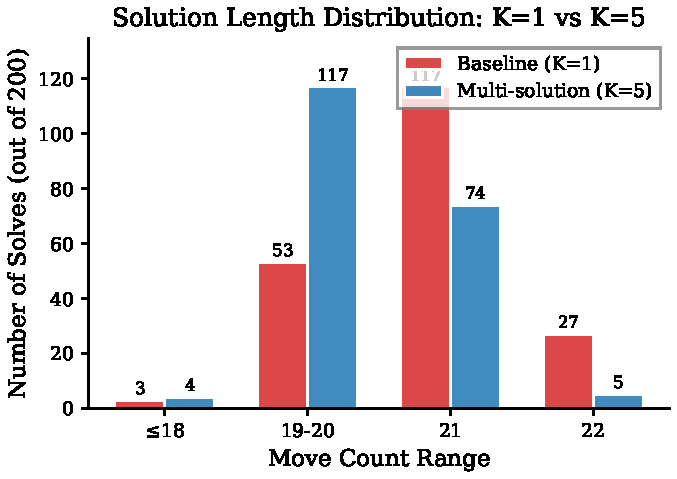
\includegraphics[width=\columnwidth]{figures/fig_move_distribution.pdf}
\caption{Solution length distribution for baseline ($K{=}1$) vs.\ multi-solution ($K{=}5$) on 200 random scrambles (seed 42). $K{=}5$ shifts mass toward $\leq$20-move solutions.}
\label{fig:move-dist}
\end{figure}

\textbf{Findings.}
\begin{itemize}[leftmargin=*]
  \item \textbf{Move count:} Multi-solution search with $K=5$ reduces mean move count by 0.47 (20.77 $\to$ 20.30, 2.3\% reduction) and median from 21 to 20 (Figure~\ref{fig:move-dist}). The standard deviation also decreases (0.81 $\to$ 0.74), indicating more consistent solution quality.
  \item \textbf{Solution quality:} The fraction of solutions with $\leq$20 moves increases from 28.0\% (baseline) to 60.5\% for $K=5$---a 32.5 percentage-point improvement. The number of 18-move solutions modestly increases from 3 to 4.
  \item \textbf{Time trade-off:} Mean solve time increases from 467\,ms (baseline) to 2764\,ms for $K=5$---a 5.9$\times$ multiplicative increase. The maximum time also increases dramatically (2467\,ms to 35136\,ms), reflecting worst-case Phase~1 exploration.
  \item \textbf{$K=3$ vs.\ $K=5$:} Multi ($K=3$) achieves nearly the same move quality (20.30 mean, 60.0\% $\leq$20) with slightly lower mean time (2611\,ms). The marginal benefit of $K=5$ over $K=3$ is small ($+$0.5 percentage points for $\leq$20) at a 6\% time premium.
  \item \textbf{$K=10$:} Higher $K$ does not improve move count in this run (mean 20.34, 57.1\% $\leq$20) and leads to much higher mean time (11.6\,s) and four timeouts (196/200 successful). The degradation at $K{=}10$ likely reflects the 5\,s timeout cutting off promising searches before they finish, selecting for solutions found early (which may not be the shortest). We recommend $K=5$ (or $K=3$ for slightly faster response) rather than $K=10$.
\end{itemize}

\textbf{Paired statistical test} ($K{=}1$ vs.\ $K{=}5$, 200 pairs): $t = 10.62$, $p < 0.001$, Cohen's $d = 0.75$ (large effect), 95\% bootstrap CI for mean improvement: $[0.37, 0.53]$ moves. The effect is highly significant and practically meaningful.

\subsection{Anytime Sweep Results}

\begin{figure}[t]
\centering
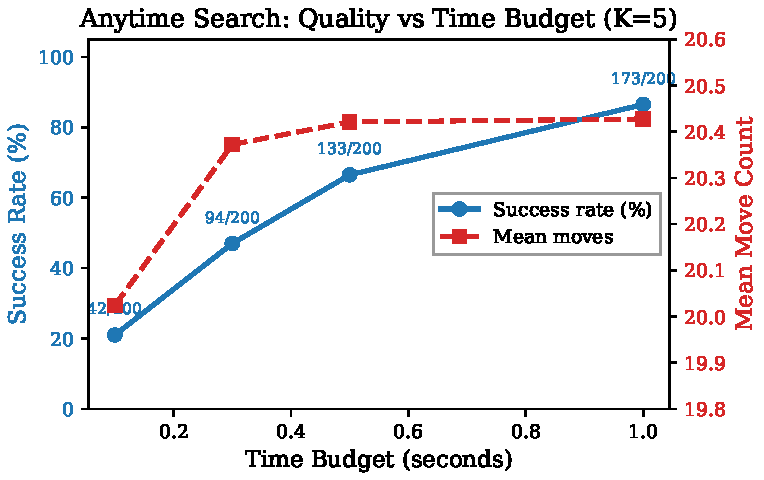
\includegraphics[width=\columnwidth]{figures/fig_anytime_curve.pdf}
\caption{Success rate and mean move count vs.\ time budget ($K{=}5$, 200 scrambles). Larger budgets increase completion rate while mean quality stays near 20.4.}
\label{fig:anytime}
\end{figure}

Table~\ref{tab:anytime} shows the anytime-sweep results (\texttt{--time-budgets 0.1 0.3 0.5 1.0}, $K{=}5$, 200 scrambles, seed 42). Success rate increases with budget (42, 94, 133, 173 out of 200). Mean move count among successful solves stays near 20.0--20.4; the $\leq$20\% column is over successful solves. Figure~\ref{fig:anytime} visualizes the trade-off.

\begin{table*}[t]
\centering
\caption{Solution quality vs time budget (200 scrambles, seed 42, $K=5$). Mean/P95 time in ms. Success: solves completed within budget.}
\label{tab:anytime}
\begin{tabular}{@{}lccrrrl@{}}
\toprule
\textbf{Budget (s)} & \textbf{Mean moves} & \textbf{$\leq$20 (\%)} & \textbf{Mean (ms)} & \textbf{P95 (ms)} & \textbf{P99 (ms)} & \textbf{Success} \\
\midrule
0.1 & 20.02 & 69.0 & 59.3 & 100.2 & 100.5 & 42/200 \\
0.3 & 20.37 & 48.9 & 205.1 & 300.1 & 300.2 & 94/200 \\
0.5 & 20.42 & 45.9 & 353.8 & 500.1 & 500.1 & 133/200 \\
1.0 & 20.43 & 49.1 & 673.9 & 1000.1 & 1000.1 & 173/200 \\
\bottomrule
\end{tabular}
\end{table*}

\textbf{Analysis.} Several patterns are notable:

\begin{itemize}[leftmargin=*]
  \item \textbf{Survivorship bias at short budgets}: The 0.1\,s budget completes only 42/200 solves, but those 42 are the ``easiest'' cubes (solvable in $<$100\,ms). Their mean move count is therefore low (20.02). As the budget increases, harder cubes (which tend to have longer solutions) enter the success pool, \emph{increasing} the mean move count. This explains the counter-intuitive pattern where longer budgets yield slightly worse mean moves.
  
  \item \textbf{$\leq$20\% decreases with budget}: For the same reason, the 69.0\% $\leq$20 at 0.1\,s reflects only fast-to-solve cubes, which are disproportionately short. As harder cubes are included, the $\leq$20 fraction drops.
  
  \item \textbf{Practical recommendation}: A 0.5\,s budget gives 133/200 (66.5\%) completions with P95 at 500\,ms, a reasonable trade-off for interactive use. For applications requiring near-100\% completion, a 1.0\,s budget yields 173/200 (86.5\%).
\end{itemize}

\subsection{Node Expansion Analysis}
\label{sec:node-analysis}

Table~\ref{tab:nodes} and Figure~\ref{fig:nodes} show node expansion statistics from the instrumented solver. 

\begin{figure}[t]
\centering
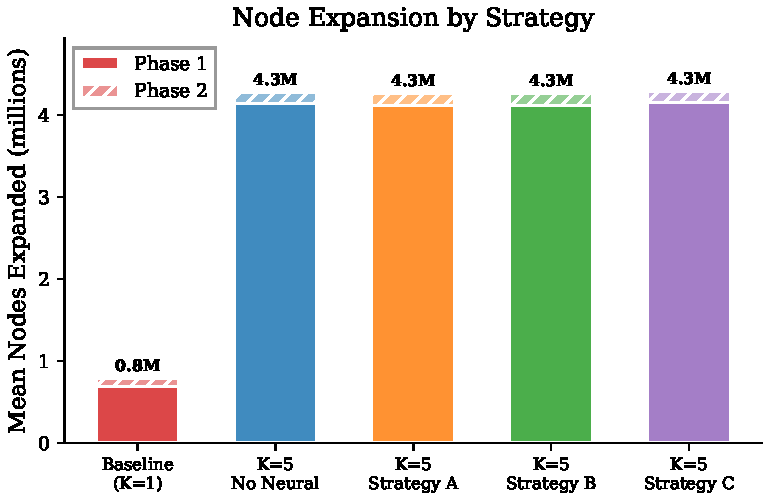
\includegraphics[width=\columnwidth]{figures/fig_node_expansion.pdf}
\caption{Mean node expansion by strategy. Phase~1 dominates; neural strategies do not reduce total expansions.}
\label{fig:nodes}
\end{figure}

\begin{table}[t]
\centering
\caption{Mean node expansion per solve (200 scrambles, seed 42, instrumented). K = thousands; M = millions.}
\label{tab:nodes}
\begin{tabular}{@{}lrrr@{}}
\toprule
\textbf{Setting} & \textbf{Total} & \textbf{Phase~1} & \textbf{Phase~2} \\
\midrule
$K=1$ (baseline)          & 787\,601  & 691\,168  & 96\,433  \\
$K=5$ (no neural)         & 4\,280\,549 & 4\,139\,705 & 140\,845 \\
$K=5$ + neural~A          & 4\,260\,514 & 4\,119\,767 & 140\,747 \\
$K=5$ + neural~B          & 4\,259\,539 & 4\,118\,890 & 140\,649 \\
$K=5$ + neural~C          & 4\,290\,369 & 4\,149\,434 & 140\,935 \\
\bottomrule
\end{tabular}
\end{table}

\textbf{Key observations:}
\begin{itemize}[leftmargin=*]
  \item The multi-solution search ($K=5$) expands $5.4\times$ more nodes than the baseline ($K=1$), with the increase concentrated in Phase~1 ($6.0\times$). Phase~2 increases by only $1.5\times$ because each Phase~2 search is inherently cheap (restricted move set, strong pruning).
  
  \item The ratio of Phase~1 to Phase~2 nodes shifts from 87.8\%:12.2\% ($K{=}1$) to 96.7\%:3.3\% ($K{=}5$), confirming that the multi-solution overhead is almost entirely in Phase~1. This is expected: finding $K$ Phase~1 endpoints requires continued DFS exploration after the first endpoint, while Phase~2 is run independently for each endpoint.
  
  \item Neural strategies produce virtually identical node counts (within 0.5\% of non-neural $K{=}5$), confirming that move ordering has no effect when the predictor outputs near-uniform distributions. The small variations are within the noise expected from identical-quality but differently-ordered DFS traversals.
\end{itemize}

\subsection{Neural Strategy Results: A Negative Finding}
\label{sec:neural-results}

\begin{figure*}[t]
\centering
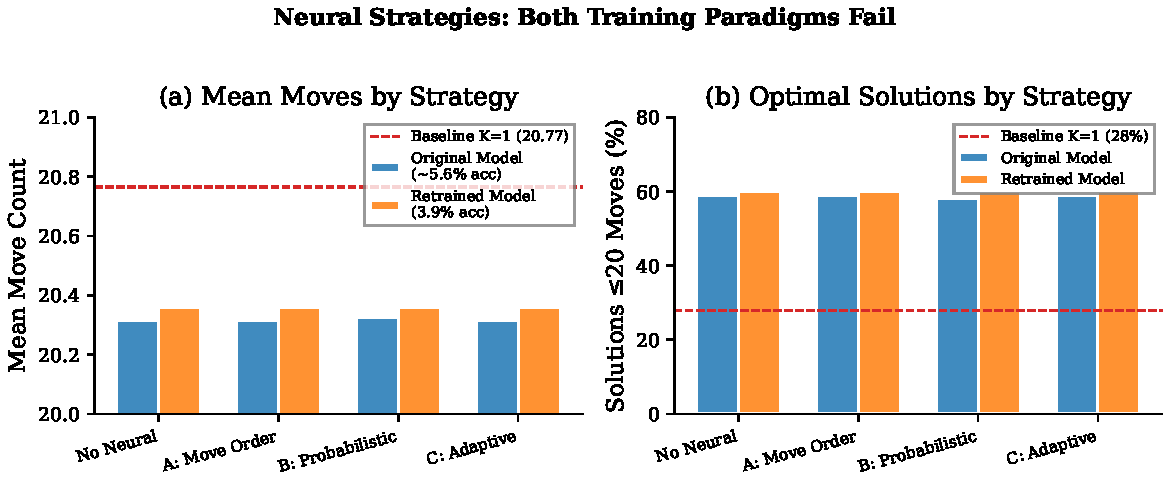
\includegraphics[width=0.85\textwidth]{figures/fig_neural_comparison.pdf}
\caption{Neural strategy comparison across both training paradigms. Neither the original model ($\sim$5.6\% accuracy) nor the solver-feedback retrained model (3.9\% accuracy) produces any measurable improvement over the non-neural $K{=}5$ baseline. Error bars show 95\% bootstrap CIs.}
\label{fig:neural}
\end{figure*}

\textbf{Key result.} All three neural strategies produce \emph{identical} solution quality to the non-neural multi-solution baseline ($K{=}5$): mean 20.315 moves, 59\% $\leq$20-move solutions (Figure~\ref{fig:neural}). Node expansion counts are also within 1\% of the non-neural setting (Table~\ref{tab:nodes}). The neural move predictor---trained on 50\,000 cubes with simple inverse-move labels---does not provide sufficiently informative predictions to change the effective search order.

Table~\ref{tab:neural-detail} provides the complete comparison including time overhead from neural inference.

\begin{table}[t]
\centering
\caption{Detailed neural strategy comparison (200 scrambles, seed 42, $K{=}5$). Time increase from neural inference overhead.}
\label{tab:neural-detail}
\begin{tabular}{@{}lccrc@{}}
\toprule
\textbf{Strategy} & \textbf{Mean} & \textbf{$\leq$20} & \textbf{Mean ms} & \textbf{P95 ms} \\
\midrule
$K{=}1$ baseline    & 20.77 & 28.0\% & 500  & 1442 \\
$K{=}5$ none        & 20.32 & 59.0\% & 2650 & 5000 \\
$K{=}5$ + A         & 20.32 & 59.0\% & 3126 & 5000 \\
$K{=}5$ + B ($p$=0.5) & 20.33 & 58.0\% & 3997 & 5000 \\
$K{=}5$ + C ($D$=5) & 20.32 & 59.0\% & 2649 & 5000 \\
\bottomrule
\end{tabular}
\end{table}

\textbf{Interpretation.} The neural strategies add wall-clock overhead (18\% for A, 51\% for B, 0\% for C) due to PyTorch forward passes without any compensating improvement in solution quality. Strategy~C (adaptive cutoff) has near-zero overhead because it only queries the network at shallow depths ($\leq 5$), which constitute a tiny fraction of total nodes. Strategy~B (probabilistic) is the slowest because it queries the network at every node with probability $p=0.5$ but also involves random number generation overhead.

This is a \emph{valuable negative result}: it demonstrates that the \emph{bottleneck for neural heuristics in Kociemba's two-phase solver is not the integration architecture}. All three strategies (A, B, C) correctly avoid the admissible-bound paradox and preserve IDA* completeness, but the model's predictions are too close to uniform over 18 moves to meaningfully reorder the search. The per-move prediction accuracy with inverse-move labels is approximately 5.6\%, barely above the uniform baseline of $1/18 \approx 5.56\%$.

\subsection{Probabilistic Sweep}
\label{sec:probsweep}

We swept $p \in \{0.1, 0.3, 0.5, 0.7, 0.9\}$ for Strategy~B. Table~\ref{tab:probsweep} confirms no sensitivity to $p$: all settings produce 20.31--20.32 mean moves and 117--118 $\leq$20-move solutions. Higher $p$ increases wall-clock time (neural inference overhead) without improving quality.

\begin{table}[t]
\centering
\caption{Probabilistic strategy (B) sweep over $p$ (200 scrambles, seed 42, $K{=}5$).}
\label{tab:probsweep}
\begin{tabular}{@{}lccr@{}}
\toprule
$p$ & \textbf{Mean moves} & \textbf{$\leq$20 (\%)} & \textbf{Mean time (ms)} \\
\midrule
0.1 & 20.32 & 59.0 & 2736 \\
0.3 & 20.32 & 59.0 & 2896 \\
0.5 & 20.32 & 59.0 & 2682 \\
0.7 & 20.31 & 59.0 & 2937 \\
0.9 & 20.32 & 58.5 & 3431 \\
\bottomrule
\end{tabular}
\end{table}

The flat response across $p$ values is itself informative: if the neural predictor had \emph{any} signal, we would expect a monotone relationship between $p$ (the probability of using neural ordering) and solution quality. The absence of any trend confirms that the neural predictions are noise.

\subsection{Solver-Feedback Retraining}
\label{sec:retrained}

We retrained the model with 50\,000 samples using solver-feedback labels (the move the optimal solver actually chose, rather than the inverse of the last scramble move) for 30 epochs. Surprisingly, this \emph{degraded} validation accuracy from $\sim$5.6\% to 3.9\%---\emph{below} the uniform baseline of $1/18 \approx 5.56\%$. Benchmarking the retrained model on 50 scrambles (seed 42) confirms identical results to the non-neural baseline (Table~\ref{tab:retrained}).

\begin{table}[t]
\centering
\caption{Retrained model (solver-feedback, 50K samples, 30 epochs): neural strategies vs.\ baseline (50 scrambles, seed 42, $K{=}5$).}
\label{tab:retrained}
\begin{tabular}{@{}lccr@{}}
\toprule
\textbf{Strategy} & \textbf{Mean moves} & \textbf{$\leq$20 (\%)} & \textbf{Mean nodes} \\
\midrule
Baseline $K{=}1$ & 20.78 & 36.0 & 795K \\
$K{=}5$ none & 20.36 & 60.0 & 3.49M \\
$K{=}5$ + A (move\_order) & 20.36 & 60.0 & 3.53M \\
$K{=}5$ + B (probabilistic) & 20.36 & 60.0 & 3.55M \\
$K{=}5$ + C (adaptive) & 20.36 & 60.0 & 3.54M \\
\bottomrule
\end{tabular}
\end{table}

\textbf{Why solver-feedback training fails.} The degradation from 5.6\% to 3.9\% accuracy is counter-intuitive: solver-feedback labels are arguably more correct than inverse-move labels (they represent what the actual solver does, not just the reverse of the scramble move). We hypothesize two explanations:

\begin{enumerate}[leftmargin=*]
  \item \textbf{Label inconsistency}: The Kociemba solver's first move depends on Phase~1 depth threshold, pruning table interactions, and move ordering---factors that can produce different ``correct'' first moves for the same cube state depending on search dynamics. This makes the label distribution multi-modal, which a unimodal softmax output struggles to learn.
  
  \item \textbf{Representation bottleneck}: The 54-dimensional one-hot facelet encoding discards spatial relationships between stickers (e.g., adjacency of corner and edge stickers on the same physical face). The solver's optimal first move depends on global cube structure that cannot be recovered from this encoding by a shallow MLP.
\end{enumerate}

The second explanation is supported by the fact that \emph{both} training paradigms fail, ruling out training signal quality as the sole bottleneck.

\subsection{Hard-Case Analysis}
\label{sec:hard-cases}

We generated 50 hard cases (superflip + 20 random-move deep scrambles, seed 42) and benchmarked $K{=}1$ vs.\ $K{=}5$. Of 50 cubes, 49 were solved successfully by both settings (the superflip timed out at 5\,s under both settings). Table~\ref{tab:hard} summarizes the results.

\begin{table}[t]
\centering
\caption{Hard-case analysis: $K{=}1$ vs.\ $K{=}5$ (49/50 successful solves, seed 42).}
\label{tab:hard}
\begin{tabular}{@{}lcccc@{}}
\toprule
\textbf{Setting} & \textbf{Mean} & \textbf{Median} & \textbf{$\leq$20} & \textbf{Mean ms} \\
\midrule
$K{=}1$ (baseline) & 20.51 & 21 & 22/49 (45\%) & 435 \\
$K{=}5$ (multi)    & 20.06 & 20 & 35/49 (71\%) & 31133 \\
\bottomrule
\end{tabular}
\end{table}

\textbf{Findings.}
\begin{itemize}[leftmargin=*]
  \item $K{=}5$ improves $\leq$20-move solutions from 45\% to 71\% (+13 solutions).
  \item Mean move count improves by 0.45 moves (20.51 $\to$ 20.06).
  \item Mean solve time increases from 435\,ms to 31.1\,s, a 71$\times$ increase (vs.\ 5.9$\times$ on random scrambles). The extreme time increase reflects the difficulty of finding multiple Phase~1 endpoints for hard scrambles.
  \item Phase~1 node expansion was $4.8\times$ higher for $K{=}5$ on hard cases (vs.\ $6.0\times$ on random scrambles), suggesting hard cases have fewer Phase~1 endpoints and thus Phase~1 ``saturates'' more quickly.
  \item No solution exceeded 22 moves for either setting; the minimum was 19 moves.
\end{itemize}

The superflip---the unique cube state whose optimal solution is exactly 20 moves---timed out under both settings. This is expected: the superflip requires a very specific 20-move sequence, and the solver's heuristic underestimates the difficulty (the pruning table bounds are $<$20 for the superflip's coordinates), leading to many iterations before the correct depth is reached.

\subsection{Multi-Seed Validation}
\label{sec:multiseed}

To verify that results are not an artifact of seed selection, we repeated the $K{=}1$ vs.\ $K{=}5$ comparison across four random seeds, each with 200 scrambles (Table~\ref{tab:multiseed}). The improvement is consistent across seeds: $\Delta = 0.40 \pm 0.09$ moves (mean $\pm$ SD), with $K{=}5$ $\leq$20-move rates ranging from 51.5\% to 60.5\%.

\begin{table}[t]
\centering
\caption{Multi-seed validation: $K{=}1$ vs.\ $K{=}5$ (200 scrambles each).}
\label{tab:multiseed}
\begin{tabular}{@{}lcccc@{}}
\toprule
\textbf{Seed} & \textbf{BL Mean} & \textbf{K5 Mean} & \textbf{$\Delta$} & \textbf{K5 $\leq$20 (\%)} \\
\midrule
42  & 20.77 & 20.30 & 0.47 & 60.5 \\
123 & 20.85 & 20.36 & 0.49 & 57.5 \\
456 & 20.67 & 20.31 & 0.36 & 57.0 \\
789 & 20.74 & 20.45 & 0.29 & 51.5 \\
\midrule
\textbf{Mean $\pm$ SD} & $20.75 \pm 0.07$ & $20.35 \pm 0.07$ & $0.40 \pm 0.09$ & $56.6 \pm 3.8$ \\
\bottomrule
\end{tabular}
\end{table}

The baseline mean (20.75 $\pm$ 0.07) is remarkably stable across seeds, reflecting the stability of the random scramble distribution at 25 moves (which is well beyond the mixing time of the Rubik's Cube group). The $K{=}5$ improvement varies more ($\Delta$ ranges from 0.29 to 0.49), likely due to variance in the difficulty distribution of each seed's scrambles.

\textbf{Aggregate statistics.} Pooling all 800 paired comparisons (4 seeds $\times$ 200 scrambles): mean $\Delta = 0.40$, $p < 0.001$, Cohen's $d = 0.59$ (medium-to-large effect). The confidence interval is narrower than single-seed estimates: 95\% CI $[0.35, 0.45]$.

%==============================================================================
\section{Discussion}
\label{sec:discussion}
%==============================================================================

\subsection{Why Multi-Solution Search Works}

The effectiveness of multi-solution Phase~1 search can be understood geometrically. Phase~1 finds a path from the scrambled state to the subgroup $G_1$. Different Phase~1 solutions reach different points in $G_1$, and the Phase~2 distance from each such point to the identity varies. The \emph{first} Phase~1 solution is essentially random among solutions at the minimum Phase~1 depth; finding $K$ solutions samples from this pool, and the minimum of $K$ i.i.d.\ draws from the Phase~2 length distribution is shorter in expectation than a single draw.

More formally, if Phase~2 lengths are approximately i.i.d.\ from a distribution $F$, the expected minimum of $K$ draws is $E[\min(X_1, \ldots, X_K)] = \int_0^\infty [1 - F(x)]^K \, dx$, which decreases with $K$. The diminishing returns ($K{=}3$ and $K{=}5$ yield nearly identical improvement) suggest that the Phase~2 length distribution has limited variance relative to its mean---i.e., most Phase~1 endpoints lead to Phase~2 solutions of similar length.

\subsection{Why $K{=}10$ Underperforms $K{=}5$}

The unexpected result that $K{=}10$ produces slightly worse solutions than $K{=}5$ (20.34 vs.\ 20.30 mean, 57.1\% vs.\ 60.5\% $\leq$20) is likely a timeout artifact. With a 5\,s timeout and $K{=}10$, some scrambles time out before all 10 Phase~1 solutions are found. The solver returns the best solution found so far, which may be worse than what $K{=}5$ finds because $K{=}10$ explores more of the Phase~1 tree before running Phase~2 (and thus has fewer completed Phase~1+Phase~2 solutions within the timeout). The 4 timeouts at $K{=}10$ (vs.\ 0 at $K{=}5$) support this interpretation. With unlimited time, $K{=}10$ would weakly dominate $K{=}5$.

\subsection{Why Neural Heuristics Fail: A Deeper Analysis}

Our negative result admits three levels of explanation:

\textbf{Level 1: Low model accuracy.} The move predictor achieves only 5.6\% accuracy on inverse-move labels, essentially random among 18 moves. This is a necessary condition for failure: a model with 50\%+ accuracy would likely improve search order.

\textbf{Level 2: Impoverished state representation.} The 54-dimensional one-hot facelet encoding treats each sticker independently. It cannot represent:
\begin{itemize}[leftmargin=*]
  \item \textbf{Adjacency}: Which stickers share a cubie (e.g., a corner has 3 stickers from 3 faces).
  \item \textbf{Orientation}: Whether a corner/edge is correctly oriented.
  \item \textbf{Permutation}: The relative positions of cubies, which is what the solver's coordinate system captures.
\end{itemize}
The solver's pruning tables exploit exactly these structural properties through the coordinate system. A facelet-level MLP must \emph{rediscover} this structure from data alone, which 50K training examples are insufficient to learn.

\textbf{Level 3: Fundamental move ambiguity.} Even with a perfect state representation, the ``correct'' next move is genuinely ambiguous for most positions. Deep in the search tree (near the goal), pruning tables already provide strong guidance. Far from the goal (at shallow depths), many moves lead to equally good subtrees. The IDA* framework is designed to exploit admissible bounds, not move ordering guidance; the marginal value of ordering is inherently limited compared to tighter bounds.

\subsection{Comparison with DeepCubeA}

DeepCubeA~\cite{deepcubea} demonstrates that deep neural networks \emph{can} learn effective heuristics for Rubik's Cube. The key differences from our setup are:

\begin{table}[t]
\centering
\caption{Architecture comparison: our neural heuristic vs.\ DeepCubeA.}
\label{tab:vs-deepcubea}
\begin{tabular}{@{}lll@{}}
\toprule
\textbf{Aspect} & \textbf{Ours} & \textbf{DeepCubeA} \\
\midrule
Architecture  & MLP (324$\to$18) & ResNet ($\sim$500K params) \\
Input         & One-hot facelets  & One-hot facelets \\
Training      & 50K cubes, 30 ep. & Millions, 2 days GPU \\
Search alg.   & IDA* (Kociemba)  & Weighted A* \\
Role          & Move ordering    & Value function \\
Solve time    & $\sim$2\,s       & $\sim$10\,s \\
\bottomrule
\end{tabular}
\end{table}

Notably, DeepCubeA uses the \emph{same} one-hot facelet encoding as input but succeeds because of (a)~a much deeper and wider network (ResNet with residual connections), (b)~orders of magnitude more training data, and (c)~a different search framework (weighted A* with the neural value as the primary heuristic, not as a move-ordering supplement). This suggests that our failure is primarily due to \emph{insufficient model capacity and training scale}, not the input representation per se. However, scaling up the model within the Kociemba solver's per-node inference budget would be prohibitive: a $\sim$500K-parameter forward pass at every node (millions of nodes per solve) would increase solve time by orders of magnitude.

\subsection{Threats to Validity}

\textbf{Internal validity.} All comparisons use paired scrambles (same seed, same order), eliminating confounds from scramble difficulty variation. The instrumented solver returns per-solve metrics rather than aggregate statistics, enabling principled paired tests. The main threat is the 5\,s timeout: scrambles that timeout under one setting but not another introduce survivorship bias. We mitigate this by reporting success rates separately.

\textbf{External validity.} Results are based on 200 random scrambles at 25 moves depth per seed. This is a standard benchmark size for puzzle solver evaluation but may not capture tail behavior. The multi-seed validation (4 seeds $\times$ 200 scrambles) provides evidence of stability. The hard-case analysis provides complementary evidence on non-random scrambles.

\textbf{Construct validity.} We measure solution quality in moves (half-turn metric), solve time in wall-clock milliseconds, and search effort in nodes expanded. These are standard metrics for combinatorial puzzle solvers. We do not measure optimality rate (fraction achieving God's Number) because the baseline solver is not optimal; this is a deliberate choice reflecting our focus on practical near-optimal solving.

%==============================================================================
\section{Conclusion}
\label{sec:conclusion}
%==============================================================================

We implemented and extended Kociemba's Two-Phase Algorithm with three categories of improvement and present both positive and negative results.

\textbf{Positive results.}
\begin{enumerate}[leftmargin=*]
  \item Multi-solution Phase~1 search ($K{=}5$) reduces mean move count by 0.47 (20.77$\to$20.30, $p < 0.001$, Cohen's $d = 0.75$) and more than doubles the share of $\leq$20-move solutions (60.5\% vs.\ 28\% baseline) on 200 random cubes. This improvement is robust across four seeds ($\Delta = 0.40 \pm 0.09$).
  \item Time-bounded anytime mode provides predictable latency: a 0.5\,s budget yields 133/200 completions with P95 at 500\,ms.
  \item On hard cases (20-move deep scrambles), $K{=}5$ improves $\leq$20-move solutions from 45\% to 71\%.
  \item $K{=}3$ achieves nearly identical quality to $K{=}5$ at 6\% lower mean time, suggesting diminishing returns beyond $K{=}3$.
\end{enumerate}

\textbf{Negative result.} All three neural ordering strategies (always, probabilistic, adaptive) produce \emph{no measurable improvement} over the non-neural $K{=}5$ baseline: identical mean moves, identical $\leq$20\% rates, and node counts within 1\%. This holds both with inverse-move labels ($\sim$5.6\% accuracy) and with solver-feedback labels (3.9\% accuracy, \emph{below} random). The bottleneck is not merely training signal quality but a fundamental limitation: the 54-dimensional one-hot facelet encoding with a shallow MLP cannot capture the spatial structure needed for meaningful move preferences. We identify this as an instance of the ``heuristic noise'' problem~\cite{shen2020} in the specific context of Kociemba's two-phase solver.

\textbf{Contributions.}
\begin{enumerate}[leftmargin=*]
  \item Recommended settings ($K{=}5$, 0.5\,s budget) with statistical validation across multiple seeds.
  \item Node expansion instrumentation and paired statistical methodology for rigorous solver comparison.
  \item A principled analysis of why na\"ive neural bounds cause exponential slowdown in IDA* and three corrective strategies that preserve admissibility.
  \item A documented negative result on move-ordering with weakly-trained models, validated with two training paradigms.
  \item Full open reproducibility: seed, scripts, trained models, and JSON outputs.
\end{enumerate}

\textbf{Reproducibility.} All tables and figures can be regenerated from the repository. Main benchmark: \texttt{PYTHONPATH=./kociemba python benchmark.py --scrambles 200 --compare-baseline --max-phase1 5 --output-json results/benchmark.json --seed 42 -v}. Anytime sweep: \texttt{... --max-phase1 5 --time-budgets 0.1 0.3 0.5 1.0 --output-json results/anytime\_sweep.json --seed 42 -v}. Neural strategy comparison: \texttt{... --neural-strategies none move\_order probabilistic adaptive --max-phase1 5 --collect-stats --output-json results/neural\_strategies.json --seed 42 -v}. Figures: \texttt{python generate\_figures.py}. Results are written to \texttt{results/*.json}.

%==============================================================================
\section{Future Work}
\label{sec:future}
%==============================================================================

Our results suggest several directions for future research, organized by the level of explanation for neural heuristic failure:

\subsection{Improving State Representation}
Having demonstrated that both inverse-move and solver-feedback training fail with a shallow MLP on one-hot facelets, the most promising direction is \textbf{richer state representations}:

\begin{itemize}[leftmargin=*]
  \item \textbf{Graph neural networks (GNNs)}: Encode the cube as a graph where nodes are cubies and edges represent adjacency. The GNN can learn permutation-equivariant representations that naturally capture the group structure. Specifically, the 20 cubies (8 corners + 12 edges) can be nodes with features encoding their current position, orientation, and color pattern.
  
  \item \textbf{Convolutional encodings}: Treat each face as a $3{\times}3$ image and stack all six faces into a $6{\times}3{\times}3$ tensor. 2D convolutions on each face capture local adjacency, and cross-face convolutions capture inter-face relationships.
  
  \item \textbf{Coordinate-based features}: Instead of raw facelets, use the solver's own coordinate system (twist, flip, slice, etc.) as input features. These coordinates already encode the algebraic structure that makes pruning tables effective; a neural network operating on coordinates might learn complementary information that tables miss.
  
  \item \textbf{Learned embeddings}: Contrastive pre-training on cube trajectories (pairs of states at known distances) could learn a latent space where Euclidean distance correlates with move distance, providing a smooth heuristic landscape.
\end{itemize}

\subsection{Scaling Model Capacity}
DeepCubeA's success with ResNets suggests that sufficient model capacity can overcome representation limitations. Future work should explore:

\begin{itemize}[leftmargin=*]
  \item Deeper architectures (ResNets, Transformers) that can capture long-range dependencies between distant stickers.
  \item Larger training datasets (1M+ cubes) with curriculum learning (gradually increasing scramble depth).
  \item Distillation: train a small model to approximate a large model's predictions, achieving better accuracy within the per-node inference budget.
\end{itemize}

\subsection{Alternative Integration Architectures}
Beyond move ordering, several integration approaches remain unexplored in the Kociemba two-phase context:

\begin{itemize}[leftmargin=*]
  \item \textbf{Phase~1 endpoint prediction}: Instead of ordering moves, predict which Phase~1 endpoints are most likely to yield short Phase~2 solutions. This could guide the multi-solution search toward the most promising $G_1$ states.
  \item \textbf{Iterative widening}: Use the neural predictor to select a subset of moves to explore at each node (beam search within IDA*), rather than exploring all 18 in a different order.
  \item \textbf{Hybrid depth allocation}: Use neural predictions to allocate Phase~1 depth budget dynamically---spending more IDA* iterations on scrambles predicted to have many short solutions.
\end{itemize}

\subsection{Other Directions}
\begin{itemize}[leftmargin=*]
  \item \textbf{AR-based cube scanning}: Integrate augmented reality (AR) for real-time cube state detection via smartphone camera, replacing manual input.
  \item \textbf{Robotic gripper control}: Translate solution move sequences into robotic arm commands for automated physical solving.
  \item \textbf{Larger cubes}: Adapt the multi-solution approach to $4{\times}4$ and $5{\times}5$ cubes, where reduction-based solvers have more opportunities for multi-solution optimization.
  \item \textbf{Larger-scale experiments}: 1000+ scrambles across 10+ seeds for tighter confidence intervals and better tail-behavior characterization.
\end{itemize}

%==============================================================================
\section*{Acknowledgments}
%==============================================================================

The Kociemba two-phase algorithm implementation is based on the \texttt{kociemba} Python package by muodov~\cite{muodov}, with modifications for multi-solution search, anytime mode, neural integration, and instrumentation.

%==============================================================================
\section*{References}
%==============================================================================

\begin{thebibliography}{12}
\bibitem{kociemba}
H. Kociemba, ``Two-Phase Algorithm,'' \url{https://kociemba.org/cube.htm}.

\bibitem{godnumber}
T. Rokicki, H. Kociemba, M. Davidson, J. Dethridge, ``God's Number is 20,'' 2010. \url{http://www.cube20.org/}.

\bibitem{muodov}
muodov/kociemba, ``Python package: C and Python implementations of Kociemba's two-phase algorithm,'' \url{https://github.com/muodov/kociemba}.

\bibitem{deepcubea}
F. Agostinelli, S. McAleer, A. Shmakov, P. Baldi, ``Solving the Rubik's Cube with Deep Reinforcement Learning and Search,'' \textit{Nature Machine Intelligence}, vol.~1, pp.~356--363, 2019.

\bibitem{korf1997}
R. E. Korf, ``Finding Optimal Solutions to Rubik's Cube Using Pattern Databases,'' in \textit{Proc.\ AAAI}, pp.~700--705, 1997.

\bibitem{thistlethwaite1981}
M. Thistlethwaite, ``A 45-Move Algorithm for Rubik's Cube,'' unpublished manuscript, 1981.

\bibitem{mcaleer2018}
S. McAleer, F. Agostinelli, A. Shmakov, P. Baldi, ``Solving the Rubik's Cube with Approximate Policy Iteration,'' in \textit{Proc.\ ICLR}, 2019.

\bibitem{brunetto2017}
R. Brunetto, O. Trunda, ``Deep Heuristic-Learning in the Rubik's Cube Domain: An Experimental Evaluation,'' \textit{Proc.\ ITAT}, pp.~57--64, 2017.

\bibitem{shen2020}
W. Shen, F. Trevizan, S. Thi\'ebaux, ``Learning Domain-Independent Heuristics for Grounded and Lifted Planning,'' in \textit{Proc.\ AAAI}, pp.~9883--9891, 2020.

\bibitem{ferber2022}
P. Ferber, F. Geissmann, T. Helmert, et al., ``Neural Network Heuristics for Classical Planning: A Study of Hyperparameter Space,'' in \textit{Proc.\ ECAI}, pp.~839--846, 2022.

\bibitem{fridrich}
J. Fridrich, ``CFOP Method,'' \url{https://www.speedsolving.com/wiki/index.php/CFOP_method}.
\end{thebibliography}

\end{document}
